% Numerical results: figures/toy/numbers_toy.txt, figures/auto/numbers_auto.txt, figures/digits/numbers_digits.txt.

\mode<article>{\maketitle}

\section{Introduction \& The Artificial Neuron}

\begin{frame}{Why Neural Networks?}
%     \begin{itemize}
%         \item \textbf{The limitation of linear models:} Linear and logistic regression compute $\hat{y} = g(\mathbf{w}^\top \mathbf{x} + b)$. They can only form straight decision boundaries or flat planes unless we \emph{manually} engineer features (polynomials, interactions).
%         \item \textbf{Manual feature engineering is hard:} In high dimensions (e.g., images with thousands of pixels, audio, text), deciding which non-linear features to create by hand is practically impossible.
%         \item \textbf{The core idea of Neural Networks:} Instead of designing features by hand, the model \textbf{learns hierarchical features automatically} from raw data through successive layers of computation.
%         % \item \textbf{Biological inspiration:} Biological brains consist of billions of interconnected neurons communicating via electrical signals. Artificial neural networks (ANNs) borrow this modular, interconnected structure.
%         \item \textbf{Biological inspiration:} Artificial units borrow their interconnected structure from networks of neurons that communicate through electrical signals.
%     \end{itemize}
    \small
    Both models use the same predictor, with intercept $b=\hat\beta_0$ and slopes $w_j=\hat\beta_j$:
    \[
        z = \mathbf{w}^{\top}\mathbf{x}+b
          = \hat\beta_0+\hat\beta_1 x_1+\cdots+\hat\beta_p x_p.
    \]
    \begin{tabular}{@{}ll@{}}
        \textbf{Linear regression} & Identity: $\hat y=g(z)=z$. \\
        \textbf{Logistic regression} & Sigmoid: $\hat p=g(z)=1/(1+e^{-z})$, so $\log\!\frac{\hat p}{1-\hat p}=z$.
    \end{tabular}
    \begin{itemize}
        \item Linear regression fits a plane. Logistic regression has a flat decision boundary at $\hat p=0.5$, where $z=0$.
        \item We can add polynomials or interactions by hand. Choosing these features becomes difficult for images, audio, or text.
        \item Neural networks learn features from data through successive layers. Their interconnected units draw inspiration from biological neurons that communicate through electrical signals.
    \end{itemize}
\end{frame}

\begin{frame}{The Four Pillars of Neural Networks}
    Every neural network, regardless of size or complexity, is built on four core concepts:
    \begin{enumerate}
        \item \textbf{Architecture:} How artificial neurons are organized into layers (input, hidden, output) and connected together.
        \item \textbf{Forward Propagation:} Pushing input data forward through the network to generate a prediction $\hat{y}$.
        \item \textbf{Loss Function:} Measuring how far the prediction $\hat{y}$ is from the ground truth target $y$.
        \item \textbf{Backpropagation \& Optimization:} Computing gradients via the calculus chain rule and updating weights via Gradient Descent to minimize the loss.
    \end{enumerate}
    \svspace{0.4em}
    We begin with the fundamental atomic building block: a \textbf{single artificial neuron}.
\end{frame}

\begin{frame}{The Building Block: An Artificial Neuron}
    \begin{center}
    \begin{tikzpicture}[
        >=Stealth,
        scale=0.88, every node/.style={transform shape},
        font=\small,
        in_node/.style={circle, draw=blue!70, fill=blue!10, thick, minimum size=20pt, inner sep=0pt},
        sum_node/.style={circle, draw=orange!80, fill=orange!15, thick, minimum size=28pt, inner sep=0pt},
        act_node/.style={rectangle, rounded corners=4pt, draw=teal!80, fill=teal!15, thick, minimum size=26pt, inner sep=3pt},
        out_node/.style={circle, draw=purple!70, fill=purple!10, thick, minimum size=20pt, inner sep=0pt}
    ]
        % Inputs
        \node[in_node] (x1) at (0, 1.3) {$x_1$};
        \node[in_node] (x2) at (0, 0.4) {$x_2$};
        \node at (0, -0.3) {$\vdots$};
        \node[in_node] (xp) at (0, -1.1) {$x_p$};
        \node[in_node, fill=gray!20, draw=gray!70] (bnode) at (0, -2.0) {$1$};

        % Summation
        \node[sum_node] (sum) at (3.4, 0) {$\sum$};
        \node[below=4pt of sum, font=\scriptsize, align=center] {Linear Combination\\$z = \mathbf{w}^\top \mathbf{x} + b$};

        % Activation
        \node[act_node] (act) at (6.2, 0) {$g(z)$};
        \node[below=4pt of act, font=\scriptsize, align=center] {Activation\\$a = g(z)$};

        % Output
        \node[out_node] (out) at (8.6, 0) {$a$};
        \node[below=4pt of out, font=\scriptsize, align=center] {Neuron\\Output};

        % Arrows
        \draw[->, thick] (x1) -- node[above, font=\scriptsize, sloped] {$w_1$} (sum);
        \draw[->, thick] (x2) -- node[above, font=\scriptsize, sloped] {$w_2$} (sum);
        \draw[->, thick] (xp) -- node[above, font=\scriptsize, sloped] {$w_p$} (sum);
        \draw[->, thick] (bnode) -- node[below, font=\scriptsize, sloped] {$b$ (bias)} (sum);

        \draw[->, thick] (sum) -- node[above, font=\scriptsize] {$z$} (act);
        \draw[->, thick] (act) -- node[above, font=\scriptsize] {$a$} (out);

        % Annotations
        \node[above=3pt of x1, font=\footnotesize\bfseries, color=blue!80] {Inputs};
        \node[above=16pt of sum, font=\footnotesize\bfseries, color=orange!80!black] {Pre-activation};
        \node[above=16pt of act, font=\footnotesize\bfseries, color=teal!80!black] {Non-linearity};
    \end{tikzpicture}
    \end{center}
    \vspace{-0.4em}
    \small
    A single neuron computes an output in two sequential steps:
    \[
        \text{1. Linear pre-activation: } z = b + \sum_{j=1}^p w_j x_j = \mathbf{w}^\top \mathbf{x} + b, \qquad
        \text{2. Activation: } a = g(z).
    \]
\end{frame}

\begin{frame}{Anatomy of an Artificial Neuron}
    \begin{itemize}
        \item \textbf{Inputs} ($x_1, \dots, x_p$): Incoming numerical features or signals from earlier layers.
        \item \textbf{Weights} ($w_1, \dots, w_p$): Learnable parameters representing connection strengths. Each weight scales how strongly an input influences the neuron.
        \item \textbf{Bias} ($b$): An intercept term that shifts the pre-activation $z$ independently of the inputs, controlling the neuron's baseline activation threshold.
        \item \textbf{Pre-activation} ($z$): The weighted sum $z = \mathbf{w}^\top \mathbf{x} + b$. This is purely linear.
        \item \textbf{Activation Function} ($g$): A non-linear function that squashes or transforms $z$ into the neuron's final activation $a = g(z)$.
    \end{itemize}
\end{frame}

\begin{frame}{Connecting Neurons to Familiar Models}
    A single neuron reproduces the classical models from earlier lectures:
    \begin{itemize}
        \item \textbf{Linear Regression:} Identity activation $g(z) = z$
        \[
            \hat{y} = \mathbf{w}^\top \mathbf{x} + b.
        \]
        \item \textbf{Logistic Regression:} Sigmoid activation $g(z) = \sigma(z) = \frac{1}{1+e^{-z}}$
        \[
            \hat{p} = \sigma(\mathbf{w}^\top \mathbf{x} + b).
        \]
    \end{itemize}
    \pause
    \svspace{0.3em}
    \textbf{The geometric limitation:}
    \begin{itemize}
        \item At cutoff $\hat{p} = 0.5$, the decision boundary satisfies $\mathbf{w}^\top \mathbf{x} + b = 0$.
        \item A single neuron can \textbf{only} create a straight line or flat hyperplane!
        \item It cannot separate curved or non-convex classes (such as XOR).
    \end{itemize}
\end{frame}

\begin{frame}{Where Does a Single Neuron Fail?}
    \begin{columns}[c]
        \begin{column}{0.50\textwidth}
            \small
            \begin{itemize}
                % \item When data has non-linear structure, a single linear boundary makes systematic errors.
                \item A straight boundary makes systematic errors on these curved classes.
                % \item The solid line shows logistic regression (a single unit): it cannot bend around the curved class boundary.
                \item The solid line is the logistic regression boundary.
                % \item In earlier lectures, we fixed this by manually inventing polynomial terms ($x_1^2, x_1 x_2$).
                \item Earlier we added polynomial features such as $x_1^2$ and $x_1x_2$ by hand.
                % \item \textbf{The solution:} Connect multiple neurons into a \textbf{network} to learn non-linear boundaries automatically!
                \item A network can learn features that bend the boundary.
            \end{itemize}
        \end{column}
        \begin{column}{0.48\textwidth}
            \centering
            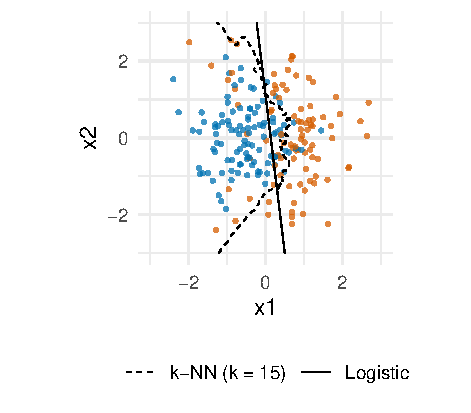
\includegraphics[width=\linewidth,height=0.36\textheight,keepaspectratio]{../06_classification/figures/cls_logistic_vs_knn.pdf}
            \par{\scriptsize Logistic regression (single unit) misses the curve.}
        \end{column}
    \end{columns}
\end{frame}


\section{Network Architecture \& Activation Functions}

\begin{frame}{Building a Network: The Multi-Layer Perceptron}
    \begin{columns}[c]
        \begin{column}{0.58\textwidth}
            \centering
            \begin{tikzpicture}[
                >=Stealth,
                scale=0.74, every node/.style={transform shape},
                font=\small,
                neuron/.style={circle, draw=blue!70, fill=blue!10, thick, minimum size=16pt, inner sep=0pt},
                hid1/.style={circle, draw=orange!80, fill=orange!15, thick, minimum size=16pt, inner sep=0pt},
                hid2/.style={circle, draw=teal!80, fill=teal!15, thick, minimum size=16pt, inner sep=0pt},
                out_n/.style={circle, draw=purple!80, fill=purple!15, thick, minimum size=16pt, inner sep=0pt}
            ]
                % Input layer
                \node[neuron] (in1) at (0, 1.2) {$x_1$};
                \node[neuron] (in2) at (0, 0.4) {$x_2$};
                \node[neuron] (in3) at (0, -0.4) {$x_3$};
                \node[neuron] (in4) at (0, -1.2) {$x_4$};
                \node[below=4pt of in4, font=\scriptsize\bfseries, color=blue!80] {Input};

                % Hidden layer 1
                \node[hid1] (h11) at (2.4, 1.5) {$h_1^{(1)}$};
                \node[hid1] (h12) at (2.4, 0.5) {$h_2^{(1)}$};
                \node[hid1] (h13) at (2.4, -0.5) {$h_3^{(1)}$};
                \node[hid1] (h14) at (2.4, -1.5) {$h_4^{(1)}$};
                \node[below=4pt of h14, font=\scriptsize\bfseries, color=orange!80!black] {Hidden 1};

                % Hidden layer 2
                \node[hid2] (h21) at (4.8, 1.0) {$h_1^{(2)}$};
                \node[hid2] (h22) at (4.8, 0.0) {$h_2^{(2)}$};
                \node[hid2] (h23) at (4.8, -1.0) {$h_3^{(2)}$};
                \node[below=14pt of h23, font=\scriptsize\bfseries, color=teal!80!black] {Hidden 2};

                % Output layer
                \node[out_n] (o1) at (7.0, 0.5) {$\hat{y}_1$};
                \node[out_n] (o2) at (7.0, -0.5) {$\hat{y}_2$};
                \node[below=24pt of o2, font=\scriptsize\bfseries, color=purple!80!black] {Output};

                % Connections
                \foreach \i in {in1,in2,in3,in4}
                    \foreach \j in {h11,h12,h13,h14}
                        \draw[->, draw=gray!40] (\i) -- (\j);

                \foreach \i in {h11,h12,h13,h14}
                    \foreach \j in {h21,h22,h23}
                        \draw[->, draw=gray!40] (\i) -- (\j);

                \foreach \i in {h21,h22,h23}
                    \foreach \j in {o1,o2}
                        \draw[->, draw=gray!40] (\i) -- (\j);
            \end{tikzpicture}
        \end{column}
        \begin{column}{0.40\textwidth}
            \small
            \begin{itemize}
                \item \textbf{Feedforward:} Information flows strictly left-to-right without feedback loops.
                \item \textbf{Dense / Fully Connected:} Every neuron connects to all neurons in the next layer.
                \item \textbf{Parameters:} Each layer $l$ has weight matrix $\mathbf{W}^{(l)}$ and bias vector $\mathbf{b}^{(l)}$.
            \end{itemize}
        \end{column}
    \end{columns}
\end{frame}

\begin{frame}{Network Building Blocks: Layers, Width, and Depth}
    \begin{itemize}
        \item \textbf{Input Layer:} Accepts the raw feature vector $\mathbf{x} \in \mathbb{R}^p$. No weights or computations here; it distributes data to the first hidden layer.
        \item \textbf{Hidden Layer(s):} Layers between input and output. They compute internal representations (learned features) from the previous layer.
        \item \textbf{Output Layer:} Delivers the final prediction (continuous response $\hat{y}$, binary probability $\hat{p}$, or class probabilities).
        \item \textbf{Width:} The number of neurons in a given layer. More width allows a layer to capture more distinct feature patterns simultaneously.
        \item \textbf{Depth:} The number of hidden layers. \textbf{Deep Learning} refers to models with multiple hidden layers stacked sequentially.
        \item \textbf{Feature Hierarchy:} Early layers learn simple patterns (edges, lines); deeper layers combine them into complex concepts (shapes, parts, objects).
    \end{itemize}
\end{frame}

\begin{frame}{Why Are Activation Functions Necessary?}
    \textbf{The Linearity Dilemma:} What happens if we omit the activation functions and use $g(z) = z$ (identity) everywhere?
    \begin{itemize}
        \item Consider a two-layer network with inputs $\mathbf{x}$:
        \[
            \mathbf{h} = \mathbf{W}^{(1)}\mathbf{x} + \mathbf{b}^{(1)}, \qquad
            \mathbf{s} = \mathbf{W}^{(2)}\mathbf{h} + \mathbf{b}^{(2)}.
        \]
        \item Substitute $\mathbf{h}$ directly into $\mathbf{s}$:
        \[
            \mathbf{s} = \mathbf{W}^{(2)}\bigl(\mathbf{W}^{(1)}\mathbf{x} + \mathbf{b}^{(1)}\bigr) + \mathbf{b}^{(2)}
            = \underbrace{\bigl(\mathbf{W}^{(2)}\mathbf{W}^{(1)}\bigr)}_{\mathbf{W}_{\text{comb}}}\mathbf{x} + \underbrace{\bigl(\mathbf{W}^{(2)}\mathbf{b}^{(1)} + \mathbf{b}^{(2)}\bigr)}_{\mathbf{b}_{\text{comb}}}.
        \]
        \item The result is still strictly a \textbf{single linear transformation}!
    \end{itemize}
    \pause
    \svspace{0.3em}
    \textbf{Key insight:} A linear combination of linear functions is always linear. A 100-layer network without non-linear activations computes nothing more than standard linear regression. Non-linear activations give networks their expressive power.
\end{frame}

\begin{frame}{Common Activation Functions}
    \begin{center}
    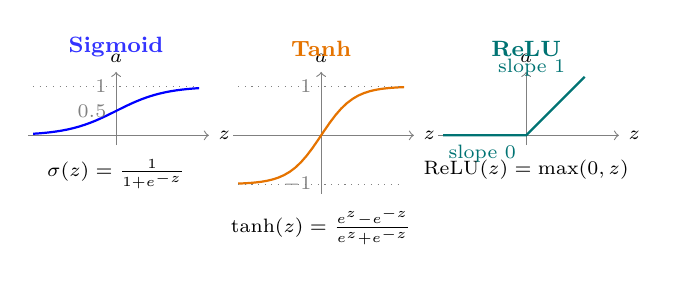
\begin{tikzpicture}[font=\scriptsize, scale=0.62]
        % Sigmoid plot
        \begin{scope}[xshift=-4.2cm]
            \draw[->, gray] (-1.8,0) -- (1.9,0) node[right, black] {$z$};
            \draw[->, gray] (0,-0.2) -- (0,1.3) node[above, black] {$a$};
            \draw[thick, blue] plot[domain=-1.7:1.7, samples=30] (\x, {1/(1+exp(-2*\x))});
            \node[below, font=\scriptsize] at (0,-0.3) {$\sigma(z) = \frac{1}{1+e^{-z}}$};
            \node[above=2pt, font=\footnotesize\bfseries, color=blue!80] at (0,1.3) {Sigmoid};
            \draw[dotted, gray] (-1.7, 1) -- (1.7, 1);
            \node[left, gray] at (0, 1) {$1$};
            \node[left, gray] at (0, 0.5) {$0.5$};
        \end{scope}

        % Tanh plot
        \begin{scope}[xshift=0cm]
            \draw[->, gray] (-1.8,0) -- (1.9,0) node[right, black] {$z$};
            \draw[->, gray] (0,-1.2) -- (0,1.3) node[above, black] {$a$};
            \draw[thick, orange!90!black] plot[domain=-1.7:1.7, samples=30] (\x, {(exp(1.5*\x)-exp(-1.5*\x))/(exp(1.5*\x)+exp(-1.5*\x))});
            \node[below, font=\scriptsize] at (0,-1.3) {$\tanh(z) = \frac{e^z - e^{-z}}{e^z + e^{-z}}$};
            \node[above=2pt, font=\footnotesize\bfseries, color=orange!90!black] at (0,1.3) {Tanh};
            \draw[dotted, gray] (-1.7, 1) -- (1.7, 1);
            \draw[dotted, gray] (-1.7, -1) -- (1.7, -1);
            \node[left, gray] at (0, 1) {$1$};
            \node[left, gray] at (0, -1) {$-1$};
        \end{scope}

        % ReLU plot
        \begin{scope}[xshift=4.2cm]
            \draw[->, gray] (-1.8,0) -- (1.9,0) node[right, black] {$z$};
            \draw[->, gray] (0,-0.2) -- (0,1.3) node[above, black] {$a$};
            \draw[thick, teal!90!black] (-1.7,0) -- (0,0) -- (1.2,1.2);
            \node[below, font=\scriptsize] at (0,-0.3) {$\mathrm{ReLU}(z) = \max(0,z)$};
            \node[above=2pt, font=\footnotesize\bfseries, color=teal!90!black] at (0,1.3) {ReLU};
            \node[above left, teal!90!black] at (1.0,1.0) {slope $1$};
            \node[below, teal!90!black] at (-0.9,0) {slope $0$};
        \end{scope}
    \end{tikzpicture}
    \end{center}
    \vspace{-0.9em}
    \small
    \begin{itemize}
        \item \textbf{Sigmoid:} Squashes to $(0, 1)$. Good for output probabilities; \textbf{saturates} for large $|z|$ (vanishing gradient: derivative $\approx 0$).
        % \item \textbf{Tanh:} Squashes to $(-1, 1)$, zero-centered. Often trains faster than sigmoid, but still saturates at extremes.
        \item \textbf{Tanh:} Squashes to $(-1, 1)$, zero-centered. Can train faster than sigmoid. Saturates at extremes.
        % \item \textbf{ReLU (Rectified Linear Unit):} Modern default for hidden layers! Extremely fast; derivative is $1$ for $z > 0$, preventing vanishing gradients.
        \item \textbf{ReLU (Rectified Linear Unit):} A common, inexpensive hidden activation. Its slope is $1$ for $z>0$ and $0$ for $z<0$. Gradients can still shrink across layers.
    \end{itemize}
\end{frame}

\begin{frame}{How ReLUs Carve Non-Linear Boundaries}
    \begin{columns}[c]
        \begin{column}{0.50\textwidth}
            \small
            \begin{itemize}
                \item A ReLU unit $h = \max(0, b + w_1 x_1 + w_2 x_2)$ is:
                \begin{itemize}\footnotesize
                    \item \textbf{Inactive} ($h=0$) when $z \le 0$.
                    \item \textbf{Active} ($h = z$) when $z > 0$.
                \end{itemize}
                \item Combining multiple units (e.g., $s = h_1 + h_2 - 1$) bends the decision boundary $s=0$ into piecewise-linear facets!
                \item More units create finer facets, enabling networks to approximate arbitrarily curved boundaries.
            \end{itemize}
        \end{column}
        \begin{column}{0.48\textwidth}
            \centering
            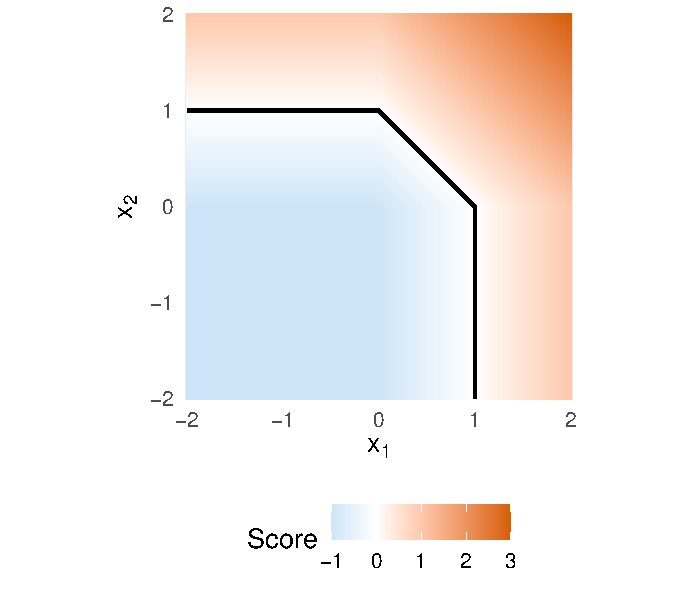
\includegraphics[width=\linewidth,height=0.42\textheight,keepaspectratio]{figures/toy/fig_score_boundary.pdf}
            \par{\scriptsize Two ReLU units combine to create a bent boundary.}
        \end{column}
    \end{columns}
\end{frame}


\section{Forward Propagation \& Loss Functions}

\begin{frame}{Forward Propagation: Layer-by-Layer}
    For an $L$-layer network, forward propagation computes predictions from input $\mathbf{x}$:
    \begin{enumerate}
        \item Set initial activation: $\mathbf{a}^{(0)} = \mathbf{x}$.
        \item For each hidden layer $l = 1, \dots, L-1$:
        \[
            \mathbf{z}^{(l)} = \mathbf{W}^{(l)} \mathbf{a}^{(l-1)} + \mathbf{b}^{(l)}, \qquad
            \mathbf{a}^{(l)} = g^{(l)}\bigl(\mathbf{z}^{(l)}\bigr).
        \]
        \item For the output layer $l = L$:
        \[
            \mathbf{z}^{(L)} = \mathbf{W}^{(L)} \mathbf{a}^{(L-1)} + \mathbf{b}^{(L)}, \qquad
            \hat{\mathbf{y}} = g^{(L)}\bigl(\mathbf{z}^{(L)}\bigr).
        \]
    \end{enumerate}
    \svspace{0.3em}
    \textbf{Vectorization:} Operations are matrix multiplications and element-wise functions, making them exceptionally fast on modern GPU hardware.
\end{frame}

\begin{frame}{Worked Example: One Forward Pass by Hand}
    \begin{center}
    \begin{tikzpicture}[x=2.2cm,y=0.75cm,>=Stealth,
        unit/.style={draw,rounded corners,fill=blue!7,inner sep=4pt}]
        \node[unit] (x1) at (0,1) {$x_1 = 2$};
        \node[unit] (x2) at (0,-1) {$x_2 = -1$};
        \node[unit,fill=orange!15] (h1) at (1.4,1) {$h_1$};
        \node[unit,fill=orange!15] (h2) at (1.4,-1) {$h_2$};
        \node[unit,fill=purple!15] (out) at (2.9,0) {$\hat p$};
        \draw[->] (x1) -- node[above, font=\scriptsize] {$1$} (h1);
        \draw[->] (x1) -- node[above, font=\scriptsize, near start] {$0$} (h2);
        \draw[->] (x2) -- node[below, font=\scriptsize, near start] {$0$} (h1);
        \draw[->] (x2) -- node[below, font=\scriptsize] {$1$} (h2);
        \draw[->] (h1) -- node[above, font=\scriptsize] {$1$} (out);
        \draw[->] (h2) -- node[below, font=\scriptsize] {$1$} (out);
    \end{tikzpicture}
    \end{center}
    \vspace{-0.5em}
    \small
    % Let hidden biases be $(0, 0)$ and output bias be $-1$. Hidden units use $\mathrm{ReLU}$; output uses sigmoid $\sigma$. Input observation: $\mathbf{x} = (2, -1)^\top$ with true class $y=1$.
    For this hand calculation we choose simple weights. Hidden biases are zero and the output bias is $-1$. For $\mathbf{x}=(2,-1)^\top$ and $y=1$, apply ReLU in the hidden layer and sigmoid at the output.
    \begin{enumerate}
        \item \textbf{Pre-activations:} $z_1 = 0 + 1(2) + 0(-1) = 2, \quad z_2 = 0 + 0(2) + 1(-1) = -1$.
        \item \textbf{Hidden features:} $h_1 = \max(0, 2) = 2, \quad h_2 = \max(0, -1) = 0$ (unit 2 is off!).
        \item \textbf{Output score:} $s = -1 + 1(h_1) + 1(h_2) = -1 + 1(2) + 1(0) = 1$.
        \item \textbf{Predicted probability:} $\hat{p} = \sigma(1) = \frac{1}{1+e^{-1}} \approx \mathbf{0.7311} \implies \text{Predict Class 1}$.
    \end{enumerate}
\end{frame}

\begin{frame}{Matching Output Layer and Loss to the Task}
    \small
    The choice of output activation and loss function depends on the prediction task:
    \begin{center}
    \footnotesize
    \begin{tabular}{@{}llll@{}}
    \toprule
    Task & Output Units & Output Activation & Training Loss \\
    \midrule
    \textbf{Regression} & $1$ continuous & Linear ($\hat{y} = z$) & Squared error: $\frac{1}{2}(y - \hat{y})^2$ \\
    \textbf{Binary} & $1$ probability & Sigmoid ($\hat{p} = \sigma(z)$) & Binary cross-entropy \\
    \textbf{Multiclass} & $K$ probabilities & Softmax ($\hat{p}_k = \frac{e^{z_k}}{\sum_j e^{z_j}}$) & Categorical cross-entropy \\
    \bottomrule
    \end{tabular}
    \end{center}
    \vspace{-0.2em}
    \textbf{Softmax intuition ($K$ classes):}
    \begin{itemize}
        \item Exponentiating $e^{z_k}$ forces all class scores to be strictly positive.
        \item Normalizing by $\sum_{j=1}^K e^{z_j}$ ensures probabilities sum to $1.0$.
        % \item Example: raw scores $(2, 1, 0) \xrightarrow{\text{softmax}} (0.67, 0.24, 0.09)$.
        \item Scores $(2,1,0)$ give probabilities $(0.67,0.24,0.09)$. Predict the class with the largest probability. For a true class $k$, the loss is $-\log(\hat p_k)$.
    \end{itemize}
\end{frame}


\section{Training \& Backpropagation}

\begin{frame}{The Neural Network Training Loop}
    \begin{center}
    \begin{tikzpicture}[
        >=Stealth,
        scale=0.82, every node/.style={transform shape},
        font=\small,
        box/.style={rectangle, rounded corners=5pt, draw=blue!70, fill=blue!8, thick, align=center, minimum width=2.6cm, minimum height=0.85cm}
    ]
        \node[box] (fwd) at (0, 1.4) {\textbf{1. Forward Pass}\\Compute $\hat{y} = f(\mathbf{x}; \mathbf{W}, \mathbf{b})$};
        \node[box, draw=red!70, fill=red!8] (loss) at (5.0, 1.4) {\textbf{2. Compute Loss}\\$L(y, \hat{y})$ measures error};
        \node[box, draw=orange!80, fill=orange!8] (back) at (5.0, -0.6) {\textbf{3. Backpropagation}\\Chain rule gives $\nabla_{\mathbf{W}} L, \nabla_{\mathbf{b}} L$};
        \node[box, draw=teal!80, fill=teal!8] (opt) at (0, -0.6) {\textbf{4. Gradient Update}\\$\mathbf{W} \leftarrow \mathbf{W} - \eta \nabla_{\mathbf{W}} L$};

        \draw[->, very thick, blue!80] (fwd) -- (loss);
        \draw[->, very thick, red!80] (loss) -- (back);
        \draw[->, very thick, orange!80] (back) -- (opt);
        \draw[->, very thick, teal!80] (opt) -- (fwd);
    \end{tikzpicture}
    \end{center}
    \vspace{-0.3em}
    \small
    Training is an iterative loop: pass observations forward, evaluate error, propagate gradients backward, and nudge weights downhill using Gradient Descent.
\end{frame}

\begin{frame}{Quantifying Error: Binary Cross-Entropy Loss}
    For a single binary observation $(y \in \{0, 1\})$ and predicted probability $\hat{p}$:
    \[
        L(y, \hat{p}) = -y\log(\hat{p}) - (1-y)\log(1-\hat{p}).
    \]
    \begin{itemize}
        \item If $y = 1$: Loss is $-\log(\hat{p})$.
        \begin{itemize}
            \item Predicting $\hat{p} = 0.7311 \implies L = -\log(0.7311) = \mathbf{0.3133}$ (small penalty).
            \item Predicting $\hat{p} = 0.1000 \implies L = -\log(0.1000) = \mathbf{2.3026}$ (severe penalty!).
        \end{itemize}
        \item The loss approaches $+\infty$ as the model assigns probability near $0$ to the true class: \textbf{confident mistakes are heavily penalized}.
        \item Averaging this loss across all training samples yields the negative log-likelihood (identical to Logistic Regression).
    \end{itemize}
\end{frame}

\begin{frame}{Backpropagation: The Chain Rule in Reverse}
    How do we know whether increasing a weight $w$ will increase or decrease the loss?
    \begin{itemize}
        \item We compute the partial derivative $\frac{\partial L}{\partial w}$ (the gradient).
        \item \textbf{The Chain Rule:} Along any connected path, slopes multiply!
        \item Consider weight $w_{11}$ (connecting $x_1$ to hidden unit 1):
        \[
            x_1 \xrightarrow{\,w_{11}\,} z_1 \xrightarrow{\,\mathrm{ReLU}\,} h_1 \xrightarrow{\,v_1\,} s \xrightarrow{\,\sigma\,} \hat{p} \longrightarrow L.
        \]
        \item Applying the chain rule backward from output to input:
        \[
            \frac{\partial L}{\partial w_{11}} =
            \underbrace{\frac{\partial L}{\partial s}}_{(\hat{p} - y)} \cdot
            \underbrace{\frac{\partial s}{\partial h_1}}_{v_1} \cdot
            \underbrace{\frac{\partial h_1}{\partial z_1}}_{\mathrm{ReLU}'(z_1)} \cdot
            \underbrace{\frac{\partial z_1}{\partial w_{11}}}_{x_1}.
        \]
    \end{itemize}
\end{frame}

\begin{frame}{Backpropagation: Numerical Trace of a Gradient}
    Evaluating each factor for our observation ($x_1=2, y=1$):
    \begin{itemize}
        \item \textbf{Output error:} $\hat{p} - y = 0.7311 - 1 = \mathbf{-0.2689}$ (score is too low!).
        \item \textbf{Outgoing weight:} $v_1 = 1$ passes the error backward.
        \item \textbf{ReLU slope:} $\mathrm{ReLU}'(2) = 1$ (unit is active, gradient passes through).
        \item \textbf{Input:} $x_1 = 2$ scales the message.
    \end{itemize}
    \[
        \frac{\partial L}{\partial w_{11}} = (-0.2689) \cdot (1) \cdot (1) \cdot (2) = \mathbf{-0.5379}.
    \]
    \pause
    \textbf{Interpretation:} The negative sign means that increasing $w_{11}$ will \textbf{decrease} the loss! In one backward sweep, backpropagation computes all gradients simultaneously.
\end{frame}

\begin{frame}{Parameter Update: Gradient Descent Step}
    Gradient points uphill (steepest increase in loss). Step \textbf{downhill}:
    \[
        w_{11}^{(\text{new})} = w_{11} - \eta\,\frac{\partial L}{\partial w_{11}}
        = 1.0 - 0.1 \times (-0.5379) = \mathbf{1.0538}.
    \]
    % Let's check the result with another forward pass:
    Change only $w_{11}$ here to isolate its effect. A full training step updates all trainable weights and biases together.
    \begin{center}
    \small
    \begin{tabular}{lrrr}
    \toprule
    State & Output Score $s$ & Predicted $\hat{p}$ & Loss $L$ \\
    \midrule
    Before update & $1.0000$ & $0.7311$ & $0.3133$ \\
    After update & $1.1076$ & $0.7517$ & $\mathbf{0.2854}$ \\
    \bottomrule
    \end{tabular}
    \end{center}
    The probability of the correct class increased, and the loss dropped!
\end{frame}

\begin{frame}{Batch vs. Stochastic vs. Mini-Batch Gradient Descent}
    How many observations do we evaluate before making a parameter update?
    \begin{itemize}
        \item \textbf{Batch Gradient Descent:} Uses all $n$ training samples for each update. Accurate gradients, but slow and memory-intensive for large datasets.
        \item \textbf{Stochastic Gradient Descent (SGD):} Updates weights after every single sample. Very fast, but gradients are noisy and fluctuate erratically.
        \item \textbf{Mini-batch SGD (Standard):} Uses small subsets (e.g., 32, 64, or 128 samples).
        \begin{itemize}
            \item Best of both worlds: smooth gradient estimates and high GPU parallelism.
        \end{itemize}
    \end{itemize}
\end{frame}

\begin{frame}{Training Terminology: Batches, Steps, and Epochs}
    Three key terms define the training schedule:
    \begin{itemize}
        \item \textbf{Batch Size ($B$):} The number of training examples evaluated in one forward and backward pass. Typically powers of two: 32, 64, 128, 256.
        \item \textbf{Iteration (Step):} One single update of all model parameters using the gradient from one mini-batch.
        \item \textbf{Epoch:} One complete pass through the entire training dataset.
        \[
            % \text{Iterations per epoch} = \frac{\text{Total training observations } n}{\text{Batch size } B}.
            \text{Iterations per epoch} = \lceil n/B \rceil \quad \text{(keep the final partial batch).}
        \]
        \item Example: With $n = 3{,}060$ training images and batch size $B = 64$, one epoch consists of $\lceil 3{,}060 / 64 \rceil = 48$ iterations.
    \end{itemize}
\end{frame}

\begin{frame}{The Learning Rate ($\eta$)}
    The learning rate is the single most critical hyperparameter in training:
    \begin{columns}[c]
        \begin{column}{0.52\textwidth}
            \begin{itemize}
                \item \textbf{Too small:} Training is painfully slow; optimization may get trapped in shallow local minima.
                \item \textbf{Too large:} Steps overshoot the minimum; loss oscillates wildly or diverges to infinity ($\mathrm{NaN}$).
                \item \textbf{Just right:} Rapid, steady convergence.
                \item \textbf{Adaptive optimizers} (Adam, RMSprop) dynamically adjust step sizes per parameter.
            \end{itemize}
        \end{column}
        \begin{column}{0.46\textwidth}
            \centering
            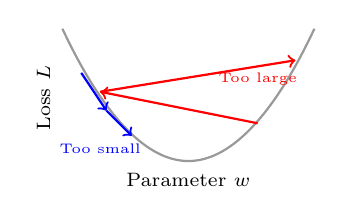
\begin{tikzpicture}[scale=0.80, font=\scriptsize]
                \draw[thick, gray!80] (-2.0, 2.3) parabola bend (0, 0.2) (2.0, 2.3);
                \node at (0, -0.1) {Parameter $w$};
                \node[rotate=90] at (-2.3, 1.2) {Loss $L$};

                % Small step
                \draw[->, blue, thick] (-1.7, 1.6) -- (-1.3, 1.0);
                \draw[->, blue, thick] (-1.3, 1.0) -- (-0.9, 0.6);
                \node[blue, font=\tiny] at (-1.4, 0.4) {Too small};

                % Overshoot
                \draw[->, red, thick] (1.1, 0.8) -- (-1.4, 1.3);
                \draw[->, red, thick] (-1.4, 1.3) -- (1.7, 1.8);
                \node[red, font=\tiny] at (1.1, 1.5) {Too large};
            \end{tikzpicture}
        \end{column}
    \end{columns}
\end{frame}


\section{Overfitting, Regularization \& Applications}

\begin{frame}{Overfitting and Network Capacity}
    \begin{columns}[c]
        \begin{column}{0.50\textwidth}
            \small
            \begin{itemize}
                \item Neural networks have high \textbf{capacity} (thousands to millions of parameters).
                \item A wide or deep network can easily memorize training noise rather than true patterns.
                \item \textbf{The Generalization Gap:} Training error keeps decreasing toward zero, but error on unseen validation data starts rising.
            \end{itemize}
        \end{column}
        \begin{column}{0.48\textwidth}
            \centering
            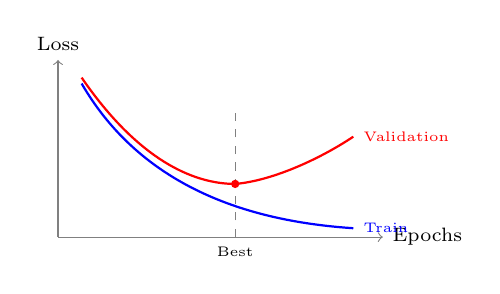
\begin{tikzpicture}[font=\scriptsize, scale=0.75]
                \draw[->, gray] (0,0) -- (5.5,0) node[right, black] {Epochs};
                \draw[->, gray] (0,0) -- (0,3.0) node[above, black] {Loss};
                % Training loss
                \draw[thick, blue] (0.4, 2.6) .. controls (1.5, 0.7) and (3.5, 0.25) .. (5.0, 0.15) node[right, font=\tiny] {Train};
                % Validation loss
                \draw[thick, red] (0.4, 2.7) .. controls (1.5, 1.1) and (2.5, 0.9) .. (3.0, 0.9) .. controls (3.6, 0.95) and (4.4, 1.3) .. (5.0, 1.7) node[right, font=\tiny] {Validation};
                % Best checkpoint
                \draw[dashed, gray] (3.0, 0) -- (3.0, 2.2);
                \node[below, font=\tiny] at (3.0, 0) {Best};
                \fill[red] (3.0, 0.9) circle (2pt);
            \end{tikzpicture}
        \end{column}
    \end{columns}
\end{frame}

\begin{frame}{Tools to Combat Overfitting}
    \begin{itemize}
        \item \textbf{Weight Decay ($L_2$ Regularization):}
        Adds a squared-weights penalty to the loss: $L_{\text{reg}} = L + \frac{\lambda}{2} \sum w_j^2$.
        Penalizes large weights, enforcing smoother decision boundaries (analogue of Ridge regression).
        \item \textbf{Dropout:}
        Randomly deactivates a fraction $p$ (e.g., $20\%$--$50\%$) of neurons during each training pass.
        Prevents neurons from co-adapting; acts like training an ensemble of subnetworks.
        \item \textbf{Early Stopping:}
        Continuously monitors validation loss after every epoch. Halts training when validation loss stops improving and saves the best model checkpoint.
    \end{itemize}
\end{frame}



% \begin{frame}{Feature Scaling: A Non-Negotiable Requirement}
\begin{frame}{How Feature Scaling Helps Training}
    \small
    % Unlike decision trees, neural networks are \textbf{critically sensitive to feature scaling}:
    Changing feature units can affect how quickly gradient descent trains a network. Tree splits depend on the ordering of feature values.
    \begin{enumerate}\footnotesize
        \item \textbf{Gradient descent efficiency:} Unscaled features produce highly eccentric loss surfaces. Gradient descent oscillates wildly and converges slowly.
        \item \textbf{Preventing vanishing gradients:} Large unscaled inputs drive pre-activations $z = \mathbf{w}^\top \mathbf{x} + b$ into flat saturation zones of Sigmoid/Tanh, where derivatives vanish ($\frac{\partial L}{\partial w} \approx 0$).
        \item \textbf{Balanced parameter updates:} Standardizing features ($\mu = 0, \sigma = 1$) or scaling to $[0, 1]$ ensures all weights update at compatible, healthy rates.
    \end{enumerate}
    \svspace{0.3em}
    % \textbf{Golden rule:} Always scale input features before training a neural network!
    \textbf{In practice:} Estimate scaling constants from the fitting data and reuse them for validation and test inputs. For digits, divide each pixel by its known maximum, 16.
\end{frame}

\begin{frame}{Regression Case Study: Auto Fuel Economy}
    \begin{columns}[c]
        \begin{column}{0.54\textwidth}
            \centering
            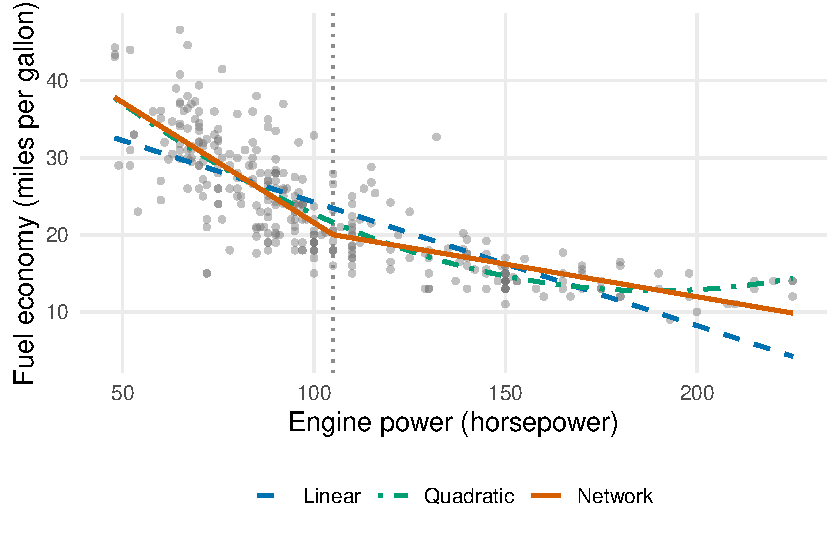
\includegraphics[width=\linewidth]{figures/auto/fig_auto_regression.pdf}
        \end{column}
        \begin{column}{0.44\textwidth}
            \small
            Predict miles per gallon (mpg) from engine horsepower using two ReLU features:
            \[
                h_L = \max(0, 105 - x),
            \]
            \[
                h_R = \max(0, x - 105).
            \]
            Linear output: $\widehat{\mathrm{mpg}} = 20.02 + 0.312\,h_L - 0.085\,h_R$.
            \svspace{0.3em}

            % The network captures the sharp bend at 105 hp.
            The fitted slopes meet at 105 hp.
        \end{column}
    \end{columns}
    \svspace{0.3em}
    \small
    % \textbf{Held-out test RMSE (79 cars):} Linear model = 4.81 mpg, Quadratic = 4.32 mpg, \textbf{Neural Network = 4.26 mpg}.
    Using 313 training cars, we tried each interior horsepower value as the bend, fitted the slopes by least squares, and chose 105 hp for its lowest squared error.\\ \textbf{Test RMSE (79 cars):} Linear 4.81, quadratic 4.32, network 4.26 mpg.
\end{frame}

\begin{frame}{Classification Case Study: Handwritten Digits}
    \begin{columns}[c]
        \begin{column}{0.50\textwidth}
            \centering
            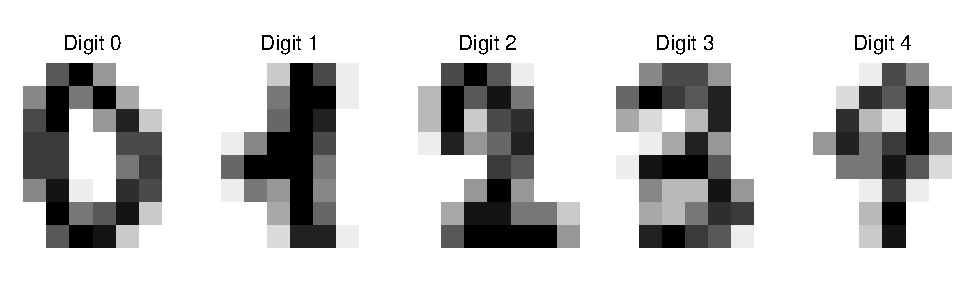
\includegraphics[width=\linewidth,height=0.45\textheight,keepaspectratio]{figures/digits/fig_training_digits.pdf}
            \par{\scriptsize 8-by-8 pixel digit images ($64$ pixels per image).}
        \end{column}
        \begin{column}{0.48\textwidth}
            \small
            \begin{itemize}
                \item \textbf{Task:} Classify $8 \times 8$ grayscale images into 10 digits ($0, \dots, 9$).
                \item \textbf{Architecture:} 64 inputs $\longrightarrow$ 32 ReLU hidden units $\longrightarrow$ 10 Softmax outputs.
                \item \textbf{Parameter counting:}
                \begin{itemize}
                    \item Hidden: $64 \times 32 + 32 = 2{,}080$.
                    \item Output: $32 \times 10 + 10 = 330$.
                    \item \textbf{Total parameters: 2,410}.
                \end{itemize}
            \end{itemize}
        \end{column}
    \end{columns}
    \small Start with small random weights so hidden units can learn different features. Use 3,060 images to fit weights, 763 to select the checkpoint, and 1,797 for the final test.
\end{frame}

\begin{frame}{Early Stopping in Practice: Handwritten Digits}
    \begin{columns}[c]
        \begin{column}{0.48\textwidth}
            \centering
            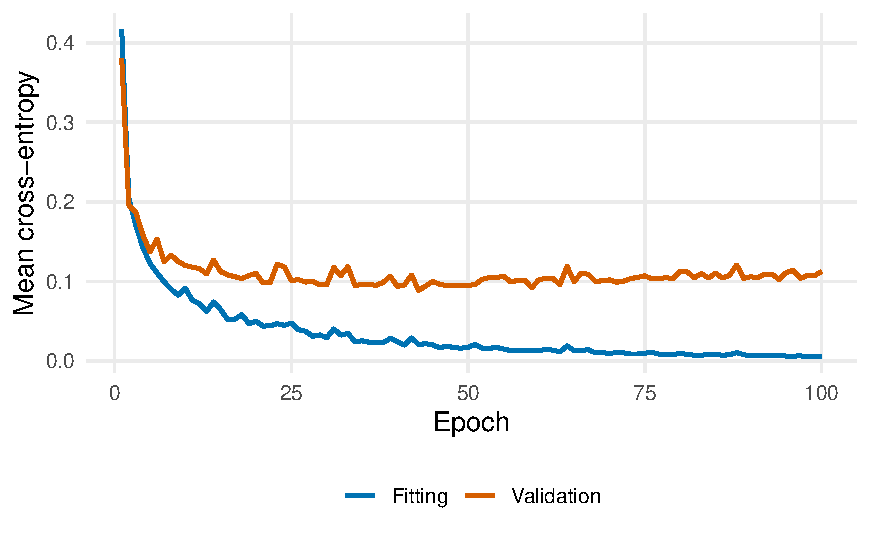
\includegraphics[width=\linewidth,height=0.42\textheight,keepaspectratio]{figures/digits/fig_learning_curves.pdf}
        \end{column}
        \begin{column}{0.50\textwidth}
            \small
            \begin{itemize}
                % \item Training an MLP on 8-by-8 digits for 100 epochs.
                \item Train for 100 epochs. Save the weights whenever validation loss reaches a new low.
                % \item Training loss (blue) drops continuously toward zero ($0.0060$).
                \item Training loss trends downward to $0.0060$.
                % \item Validation loss (red) reaches minimum of \textbf{0.0886} at \textbf{epoch 43}.
                \item Validation loss is lowest at epoch \textbf{43} ($0.0886$).
                % \item Beyond epoch 43, validation loss creeps up ($0.1122$ at epoch 100).
                \item At epoch 100, validation loss is higher ($0.1122$).
                % \item \textbf{Early stopping} restores weights at epoch 43.
                \item Restore the epoch-43 weights for the final test.
            \end{itemize}
        \end{column}
    \end{columns}
\end{frame}

\begin{frame}{Digits Performance: Baseline vs. Neural Network}
    % We compare multinomial logistic regression (linear baseline) with the 32-unit MLP on 1,797 held-out test images:
    Test results on 1,797 images for multinomial logistic regression and the 32-unit network:
    \begin{center}
    \small
    \begin{tabular}{@{}lrrr@{}}
    \toprule
    Model & Test Accuracy & Mean Log Loss & Test Errors \\
    \midrule
    % Multinomial Logistic (Baseline) & 95.21\% & 0.1846 & 86 \\
    Multinomial logistic & 95.21\% & 0.1846 & 86 \\
    \textbf{Neural Network (32 units)} & \textbf{95.88\%} & \textbf{0.1575} & \textbf{74} \\
    \bottomrule
    \end{tabular}
    \end{center}
    \begin{itemize}
        \item The neural network makes \textbf{12 fewer mistakes} on the test set.
        % \item \textbf{Accuracy vs. Log Loss:} Beyond accuracy, the network assigns higher confidence to correct classes, significantly reducing mean log loss from $0.1846$ to $0.1575$.
        \item Mean log loss falls from $0.1846$ to $0.1575$. On average, the network incurs a smaller penalty for the probability it assigns to the true digit.
    \end{itemize}
\end{frame}

\begin{frame}{Where Does the Network Make Mistakes?}
    \begin{columns}[c]
        \begin{column}{0.44\textwidth}
            \centering
            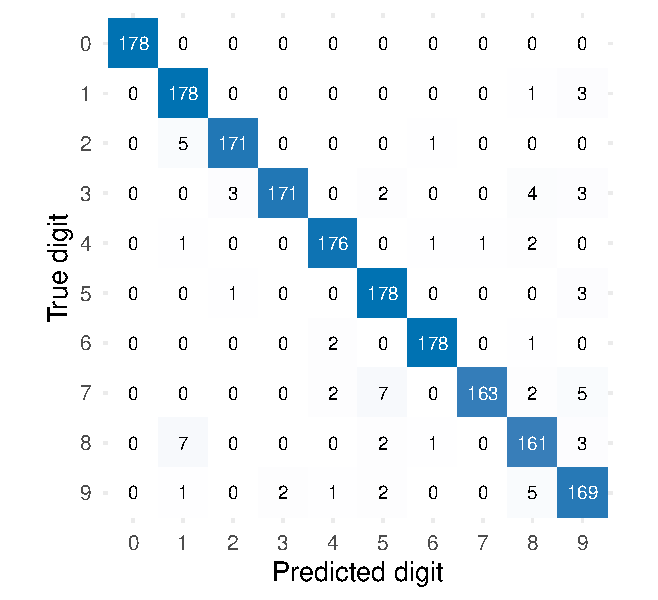
\includegraphics[width=\linewidth,height=0.42\textheight,keepaspectratio]{figures/digits/fig_confusion.pdf}
        \end{column}
        \begin{column}{0.54\textwidth}
            \centering
            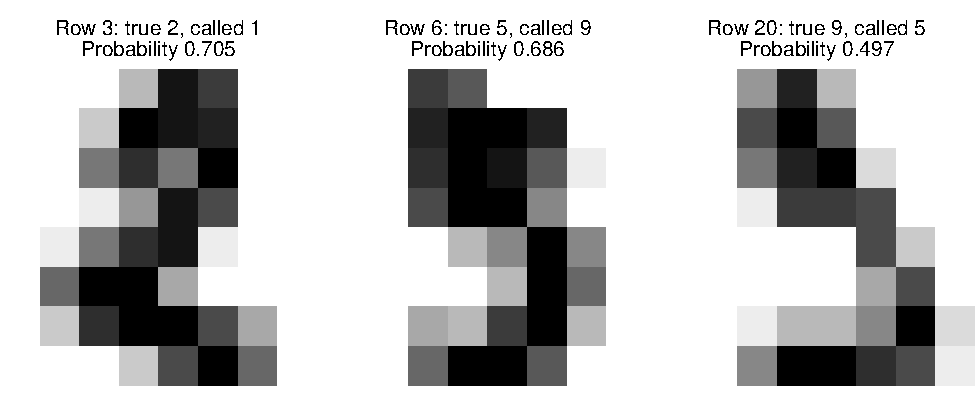
\includegraphics[width=\linewidth,height=0.15\textheight,keepaspectratio]{figures/digits/fig_test_examples.pdf}
            \small
            \begin{itemize}
                \item \textbf{Confusion matrix:} Rows are true labels; columns are predictions. Most errors involve visually ambiguous shapes (e.g., true 7s misread as 5s).
                \item In the first mistake shown, a true 2 is predicted as a 1: a heavy vertical stroke dominates the image, mimicking the stem of a 1.
            \end{itemize}
        \end{column}
    \end{columns}
\end{frame}

% \begin{frame}{Unsupervised Representation Learning: Autoencoders}
\begin{frame}{Optional: Unsupervised Learning with Autoencoders}
    \begin{columns}[c]
        \begin{column}{0.60\textwidth}
            \small
            \textbf{What if we don't have labels $y$?}
            \begin{itemize}\setlength{\itemsep}{0pt}
                \item An \textbf{autoencoder} is trained to predict its own input:
                \par\noindent\(
                    \mathbf{x} \xrightarrow{\text{Encoder}} \mathbf{h} \xrightarrow{\text{Decoder}} \hat{\mathbf{x}}.
                \)\par
                \item The hidden layer $\mathbf{h}$ has lower dimension than $\mathbf{x}$ (the \textbf{bottleneck}).
                % \item The network compresses 64 pixels into a compact code and reconstructs them.
                \item For digits, decode the compact code back into 64 pixel values.
                % \item \textbf{Connection to PCA:} A linear autoencoder with squared error recovers the exact PCA subspace!
                \item \textbf{Connection to PCA:} For centered data, a linear bottleneck trained to minimum squared reconstruction error recovers a principal subspace.
            \end{itemize}
        \end{column}
        \begin{column}{0.38\textwidth}
            \centering
            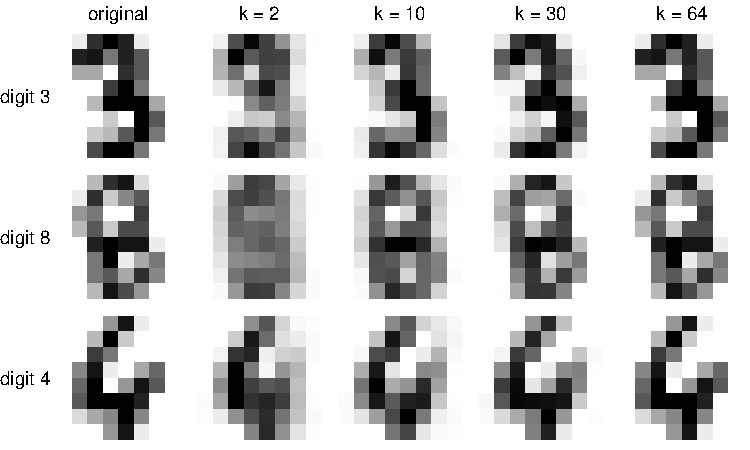
\includegraphics[width=\linewidth,height=0.35\textheight,keepaspectratio]{../12_dimensionality-reduction_pca/figures/digits/fig_digits_reconstruction.pdf}
            \par{\scriptsize PCA reconstructions from Lecture 12.}
        \end{column}
    \end{columns}
\end{frame}

\begin{frame}{Summary: Core Building Blocks of Neural Networks}
    \begin{columns}[T]
        \begin{column}{0.48\textwidth}
            \textbf{Architectural Blocks:}
            \begin{itemize}\footnotesize
                \item \textbf{Neuron:} $z = \mathbf{w}^\top \mathbf{x} + b \to a = g(z)$.
                \item \textbf{Layers:} Input, hidden, output; Width and Depth.
                \item \textbf{Non-Linearity:} Activations (ReLU, Tanh, Sigmoid) prevent network collapse.
            \end{itemize}
        \end{column}
        \begin{column}{0.48\textwidth}
            \textbf{Learning Blocks:}
            \begin{itemize}\footnotesize
                \item \textbf{Forward Pass:} Layer-by-layer computation.
                \item \textbf{Backpropagation:} Chain rule yields exact parameter gradients.
                \item \textbf{Optimization:} Mini-batch SGD with step size $\eta$.
                \item \textbf{Regularization:} Weight decay, dropout, early stopping prevent overfitting.
            \end{itemize}
        \end{column}
    \end{columns}
\end{frame}

\begin{frame}{Check Your Understanding}
    \small
    \begin{enumerate}
        % \item \textbf{Why does an MLP need non-linear activations?} \pause A composition of linear functions is strictly linear; without non-linearities, stacking 50 layers computes nothing more than a single linear regression.
        \item \textbf{Why does an MLP need non-linear activations?} \pause Even 50 layers with identity activations reduce to one weighted sum plus a bias.
        % \item \textbf{Why is ReLU preferred over Sigmoid in deep hidden layers?} \pause Sigmoid saturates at extreme values, causing gradients to vanish ($\approx 0$); ReLU maintains a derivative of $1$ for all positive inputs.
        \item \textbf{Why is ReLU preferred over Sigmoid in deep hidden layers?} \pause Sigmoid slopes approach zero at the extremes. ReLU has slope $1$ for positive inputs.
        % \item \textbf{What is the difference between an epoch and an iteration?} \pause An iteration is a single gradient update on one mini-batch; an epoch is one full pass through the entire training dataset.
        \item \textbf{What is the difference between an epoch and an iteration?} \pause One iteration updates the weights. One epoch uses all training observations.
        % \item \textbf{Which dataset determines when to stop training?} \pause Validation data. Training continues until validation error reaches its minimum, avoiding overfitting.
        \item \textbf{Which data select the checkpoint?} \pause Validation data. Keep the weights with the lowest observed validation loss.
        \item \textbf{Softmax check:} For $(0.67,0.24,0.09)$, which class wins? If the second class is correct, what is the loss? \pause The first class wins. The loss is $-\log(0.24)\approx1.43$.
    \end{enumerate}
\end{frame}
